%% Graphical abstract for "Observation Theory" (IEEE Transactions on Information Theory).
%% Standalone; compiles to a self-contained landscape PDF suitable for the graphical-
%% abstract slot. pdflatex graphical-abstract.tex
\documentclass[border=8pt]{standalone}
\usepackage[T1]{fontenc}
\usepackage{amsmath,amssymb}
\usepackage{tikz}
\usetikzlibrary{arrows.meta,positioning,fit,backgrounds,calc}
\newcommand{\PC}{P_{\mathcal{C}}}
\newcommand{\Sd}{\Sigma_{\delta}}
\newcommand{\tr}{\operatorname{tr}}
\newcommand{\dO}{d_{\mathcal{O}}}

\begin{document}
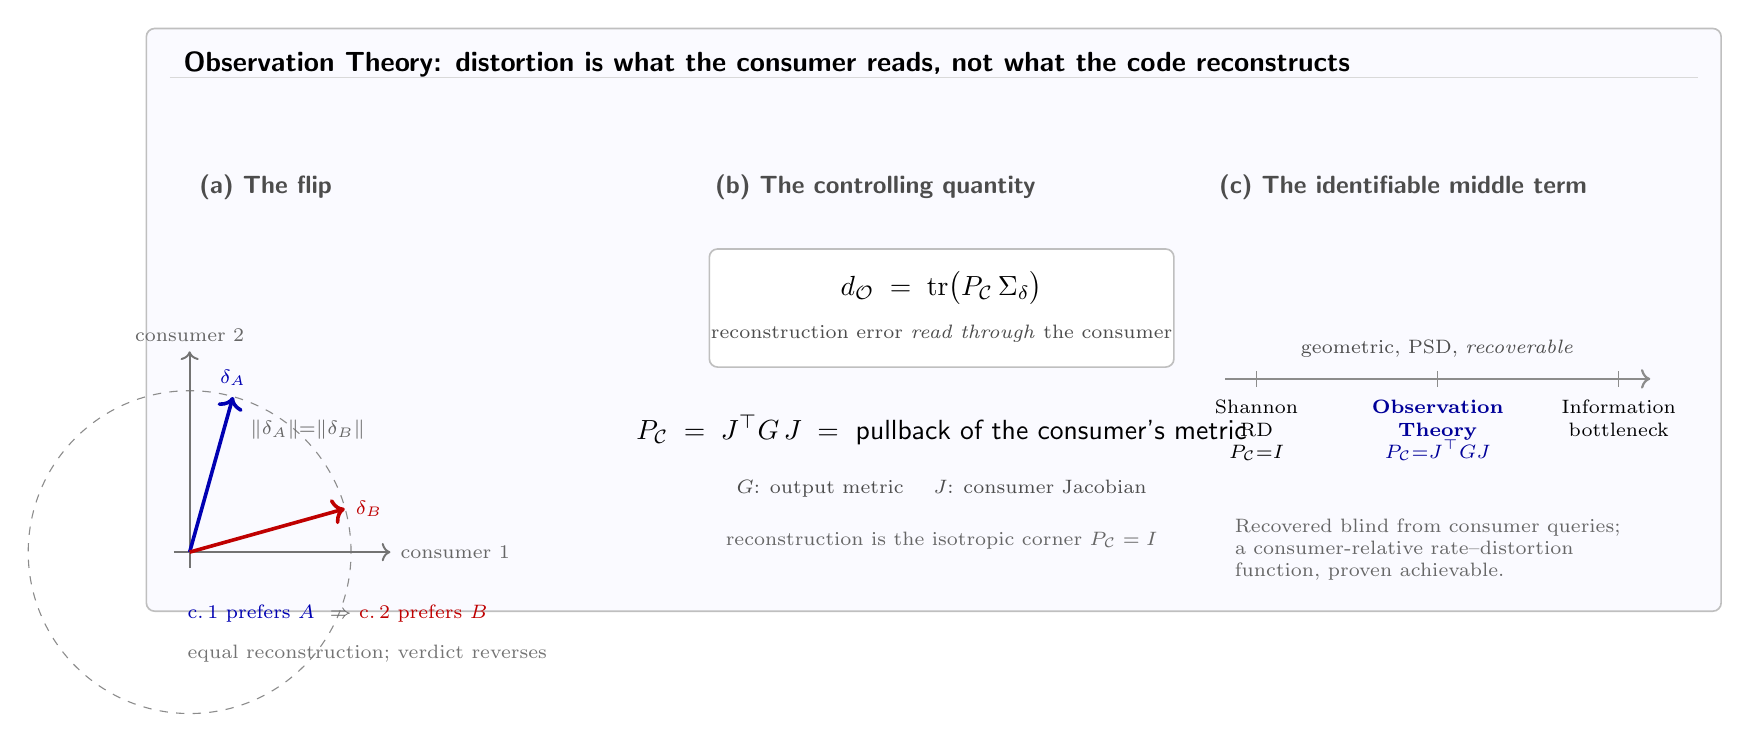
\begin{tikzpicture}[font=\sffamily,
  panel/.style={draw=black!25, rounded corners=3pt, line width=0.6pt},
  hd/.style={font=\sffamily\bfseries\small, black!70}]

% ===== overall frame width ~ 20cm, height ~ 7.2cm =====
\def\W{20} \def\H{7.4}
\node[panel, minimum width=\W cm, minimum height=\H cm, fill=blue!2] (frame) at (\W/2,\H/2) {};
\node[font=\sffamily\bfseries, anchor=north west] at (0.35,\H-0.18)
  {Observation Theory: distortion is what the \emph{consumer} reads, not what the code reconstructs};
\draw[black!15] (0.3,\H-0.62)--(\W-0.3,\H-0.62);

% ============ PANEL 1: the flip ============
\begin{scope}[shift={(0.55,0.55)}]
  \node[hd, anchor=south west] at (0,4.55) {(a) The flip};
  \coordinate (O) at (0,0.2);
  \draw[black!45,dashed] (O) circle (2.05);
  \draw[->,black!55,line width=0.7pt] ($(O)+(-0.2,0)$)--($(O)+(2.55,0)$) node[right,font=\scriptsize,black!60]{consumer 1};
  \draw[->,black!55,line width=0.7pt] ($(O)+(0,-0.2)$)--($(O)+(0,2.55)$) node[above,font=\scriptsize,black!60]{consumer 2};
  \draw[->,blue!70!black,line width=1.3pt] (O)--($(O)+(0.55,1.97)$) node[above,font=\scriptsize]{$\delta_A$};
  \draw[->,red!75!black,line width=1.3pt]  (O)--($(O)+(1.97,0.55)$) node[right,font=\scriptsize]{$\delta_B$};
  \node[font=\scriptsize,black!60,align=center] at ($(O)+(1.5,1.55)$){$\|\delta_A\|{=}\|\delta_B\|$};
  \node[font=\scriptsize,align=left,anchor=north west] at ($(O)+(-0.15,-0.55)$)
    {\color{blue!70!black}c.\,1 prefers $A$\ \ \color{black!60}$\Rightarrow$\ \color{red!75!black}c.\,2 prefers $B$};
  \node[font=\scriptsize,black!55,anchor=north west] at ($(O)+(-0.15,-1.05)$){equal reconstruction; verdict reverses};
\end{scope}

% ============ PANEL 2: the controlling quantity ============
\begin{scope}[shift={(7.1,0.55)}]
  \node[hd, anchor=south west] at (0,4.55) {(b) The controlling quantity};
  \node[panel, fill=white, minimum width=5.9cm, minimum height=1.5cm] (eq) at (3,3.3) {};
  \node at (3,3.55) {$\displaystyle \dO \;=\; \tr\!\big(\PC\,\Sd\big)$};
  \node[font=\scriptsize,black!70] at (3,2.98) {reconstruction error \emph{read through} the consumer};
  \node at (3,1.75) {$\displaystyle \PC \;=\; J^\top G\, J \;=\;$ pullback of the consumer's metric};
  \node[font=\scriptsize,black!70,align=center] at (3,1.0)
    {$G$: output metric \quad $J$: consumer Jacobian};
  \node[font=\scriptsize,black!60,align=center] at (3,0.35)
    {reconstruction is the isotropic corner $\PC=I$};
\end{scope}

% ============ PANEL 3: positioning ============
\begin{scope}[shift={(13.5,0.55)}]
  \node[hd, anchor=south west] at (0,4.55) {(c) The identifiable middle term};
  \draw[->,black!45,line width=0.8pt] (0.2,2.4)--(5.6,2.4);
  \foreach \x in {0.6,2.9,5.2} \draw[black!45] (\x,2.5)--(\x,2.3);
  \node[align=center,font=\scriptsize,anchor=north] at (0.6,2.25){Shannon\\ RD\\ $\PC{=}I$};
  \node[align=center,font=\scriptsize\bfseries,anchor=north,text=blue!60!black] at (2.9,2.25){Observation\\ Theory\\ $\PC{=}J^\top G J$};
  \node[align=center,font=\scriptsize,anchor=north] at (5.2,2.25){Information\\ bottleneck};
  \node[align=center,font=\scriptsize,black!70,anchor=south] at (2.9,2.55){geometric, PSD, \emph{recoverable}};
  \node[font=\scriptsize,black!60,anchor=north west,align=left] at (0.2,0.75)
    {Recovered blind from consumer queries;\\ a consumer-relative rate--distortion\\ function, proven achievable.};
\end{scope}

\end{tikzpicture}
\end{document}
